\section{Implementation}
\label{sec:imp}

\subsection{Individual Argos Simulations}

We use Argos to virtually test different neural network weight configurations, as described in Figure~\ref{fig:nnet}. 
We create a BUZZ template file with the weights defined as the top as \texttt{W1 = \{W1\}} etc.
This allows our python program (discussed in Section~\ref{sec:nov}) to replace these values for each population.
For exaple, if the current population has the weights \texttt{[0.1, 0.2, 0.3, 0.4, 0.5, 0.6]}, then the first weight in this file will be replaced with 0.1, the second weight will be replaced with 0.3 and so on. 
Argos will then be able to use this newly created buzz controller to control the behavior for each robot. 

The `'neural network'` code is implemented with if statements. 
If a bot detects a robot in front of it with the \emph{same} group type, it will set the wheel speed of its left wheel to $weight_1 \times K$ and the right wheel to $weight_2 \times K$ where $K$ is a constant scaling factor. 
Similarly, if the robot sees a robot of a \emph{different} type directly in front of it, it will set the left wheel speed to $weight_3 \times K$ and the right to $weight_4 \times K$. 
Finally, if no robot is seen, then the current bot will set the left wheel to $weight_5 \times K$ and the right to $weight_6 \times K$. 
This implementation is identical to the vectorized version discussed in the introduction. 

Each of the simulations will run for 5,000 time steps. 
At each time step, we record the position and wheel speeds of each bot for the current iteration. 
Further processing of these values is done in in the python code discussed in Section~\ref{sec:nov}.

\subsection{Novelty Search}
\label{sec:nov}

Our novelty search implementation closely that of Brown et. al.~\cite{c1}.
We implement this algorithm, previously shown in Figure~\ref{fig:alg}, in Listing~\ref{lst:search}.
This follows an identical layout - first, a seed population is chosen with uniform weights (although we did experiment with an intentionally `'good'` seed population which we believed would already shown some group segregation). 
On each iteration, the current most-fit population is permuted.
This means that each weight is either increased or decreased and a new population is created from this mutation(discussed further in Section~\ref{sec:time}).
Then, each of these new populations is simulated in Argos and the locations at each time-step are recorded.

After each simulation, we create a \emph{behavior vector} similar to Brown et. al. (Figure~\ref{fig:vec}).
This is to summarize the performance of each population so that we can evaluate the novelty of the parameter weights. 

\begin{figure}
    \centering
    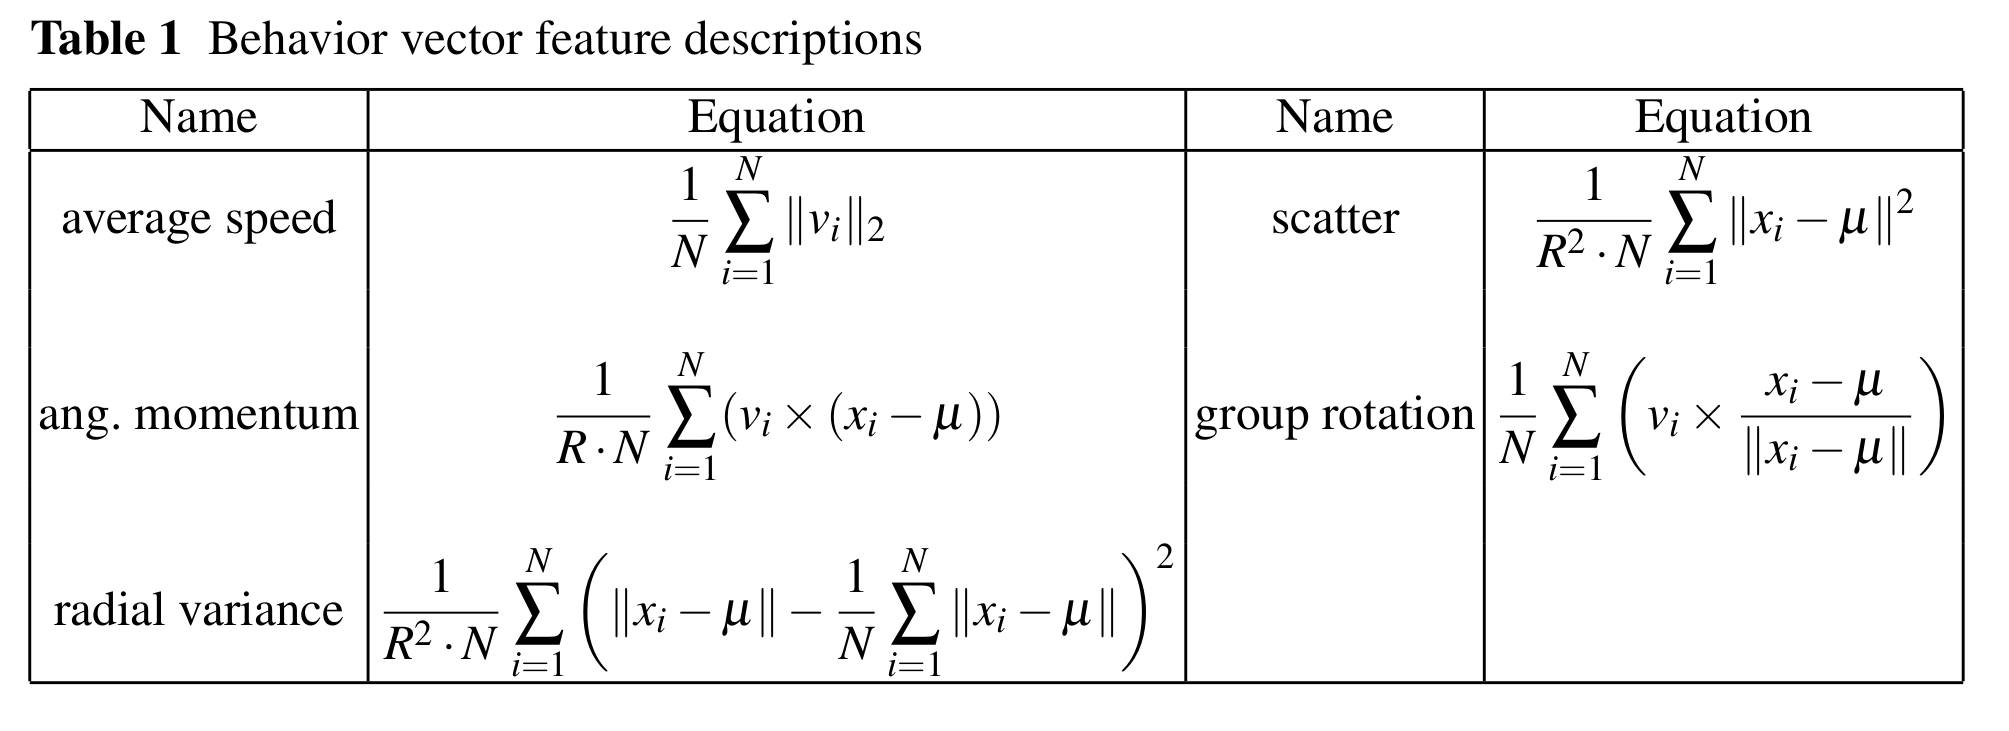
\includegraphics[width=\linewidth]{imgs/measures.png}
    \caption{Behavior Vector, Table 1 in Brown et. al.\cite{c1}}
    \label{fig:vec}
\end{figure}

\begin{lstlisting}[caption={Search algorithm (Python)}, label={lst:search}, language=Python, breaklines=true]

# Details at 
# github.com/SaahilClaypool/swarm_novelty_search/blob/master/search.py
def search():
    print("iteration, population, weights, segregation")
    seed = Observation([0.5, 0.5, 0.5, .5, .5, .5])
    population = [seed]
    archive = []
    stop = False
    it = 0
    max_it = 100
    while(max_it != 0):
        it += 1
        max_pop = -1
        for idx, p in enumerate(population):
            _features = p.getMeasures()
            global PRIOR_WEIGHTS
            PRIOR_WEIGHTS.append(p.weights)
            if (shouldAddToArchive(p, p, archive)):
                archive.append(p)

        population = updatePopulation(population, archive)

        max_it -= 1

    seg = most_segregated(archive)
    print("most segregated\n", seg)

\end{lstlisting}

\subsection{Time Complexity}
\label{sec:time}

The obstacle in our implementation is the time complexity involved in the evoluationary search.
By increasing the number of weights in our model from 4 to 6, we increased the search space from 4 dimmensions to 6. 
In our original implemntation, we were fully permutating each weight vector.
That is, for each population we would test \emph{all possible combinations} of increased or decreasing the weights in the vector. 
For example, if the weights of a two dimmensional vector were \texttt{[.1, .2]}, and the step size\footnote{We use a step size of .1, and bound each weight between 0 and 1.}, then a single permutation of this population would create the following new populations
\begin{itemize}
    \item \texttt{[.0, .1]}
    \item \texttt{[.0, .2]}
    \item \texttt{[.0, .3]}
    \item \texttt{[.1, .1]}
    \item \texttt{[.1, .3]}
    \item \texttt{[.2, .1]}
    \item \texttt{[.2, .2]}
    \item \texttt{[.2, .3]}
\end{itemize}

Which is $3^2 - 1 = 8$ new populations. 
This is because each value can either increase, decrease, or stay the same. 
So, for each new weight added, three new populations can be generated. 
This meant that when we created a 6-weight neural network, each population could generate a potential of $3^6 - 1$ populations, or 728 new populations.
Each population takes roughly 10 to 30 seconds to simulate in our implementation, causing each generation of the evolutionary search to take roughly 6 hours on a relatively powerful machine. 

Thus, we needed to adjust our implementation to reduce this time complexity. 
We did this with two different approaches. 
Our first approach was to return to a 4 weight model, but change the semantics of our simulation such that weights 1 and 2 were used only if a robot of the \emph{same} time was visible directly infront of the current robot.
Otherwise, the other two weights would be used whether there was no robot infront of the current robot, or a robot of the other type. 
This made the bots effectively blind to bots of the wrong type, but from our experimenting, it seems that well-segregated swarms would often just turn away from swarms of the oher type.
Thus, the swarms of the other type would not be in `line of sight' for more than a single time step, and thus the weights controlling the behavior when a bot of the other type is visible were rarely used. 
So, we combined these weights with the weights controlling the behavior when no bot is visible. 

Our second heuristic was to \emph{not} compute all combinations of the weights for the current population, but rather just increase each weight individually to create new populations. 
This reduces the number of new populations generated each generation from $3^W - 1$ to $3 \times W - 1$. 
In the case of our 6-weight example, this reduces the number of permutations from 728 to just 17. 
This makes each generation less effective, but made each iteration exponentially faster. 
This allowed us to run the same experiment with all 6 weights being evaluated. 
In the results, we will discuss the differences discovered by these two approaches.


\subsubsection{Fitness Search vs Novelty Search}

Unlike Brown et. al., we do not aim to categorize the complete set of possible behaviors given a limited capability model. 
Rather, we aim to answer just one question: given this capability model (4 to 6 neuron network, differential drive motor, binary line of sight, same-swarmm detection) is the behavior of segregation possible. 
Thus, a novelty is not necessarily the best fitness function - novelty is useful for ensuring our algorithm covers all parts of the search space, but that is not our aim. 
Thus we also implement a second search that replaces novelty with a traditional fitness function.
The semantics of the algorithm are unchanged. 
The only change is as follows: rather than selecting the most unique population to permutate in the next generation, we instead choose the population which exhibited the highest levels of segregation.


\subsection{Segregation Metrics}

To evaluate which population exhibited the highest levels of segregation, we created a quantifiable measure of segregation. 
To be a valid measure of segregation, this measure should have the following properties: 
\begin{itemize}
    \item Higher segregation should correspond to higher segregation measure scores

        For ease of interpretability, the measure should \emph{maximize} segregation when two groups are completely split.

    \item Groups with low segregation scores should correspond to groups that are indistinguishable from each other

        If two groups were to not segregate, that would likely mean they were interspersed evenly within each other. 
        Similarly, if two groups are interspersed evenly within each other, they are not segregated. 

\end{itemize}

Thus, the metric we use is as follows:

$$
-({\frac{DistanceDeviation_1 + DistanceDeviation_2}{2 DistanceDeviation}})
$$

Where the distance $DistanceDeviation$ is the standard deviation of all the bots to the mean position of all of the bots, $DistanceDeviation_1$ is the standard deviations of the distance of all the bots to the center of mass of that group, and $DistanceDeviation_2$ is the same for group 2. 

The reasoning for this measure is that, when the groups are overlapping, the standard deviation within a single group should be the same as the standard deviation of the entire set of robots. 
Thus the term $\frac{DistanceDeviation_1 + DistanceDeviation_2}{2 DistanceDeviation}$ should be roughly equal to 1. 
But, when the groups are highly segregated, $DistanceDeviation_1$ and $DistanceDeviation_2$ should be smaller than $DistanceDeviation$. 
Thus, the term should tend towards zero. 
Because we take the negative of this value, this measure should get larger when the bots are segregated. 
We provide validation and discussion on this measure of segregation in the next section.
